\documentclass{vldb}

\usepackage[utf8]{inputenc}

\usepackage{graphicx}
\usepackage{url}
\usepackage{hyperref}
\usepackage{algorithm} % for algorithms
\usepackage{algpseudocode}
% \usepackage{booktabs} % For formal tables

\usepackage{balance}  % for  \balance command ON LAST PAGE  (only there!)
\usepackage{caption}
\usepackage{subcaption}
\usepackage{tikz}
\usetikzlibrary{backgrounds, calc, positioning, fit, decorations.pathreplacing}
% \theoremstyle{remark}

\pagestyle{empty} % removes running headers

\newcommand{\PicScale}{0.5}
\newcommand {\FlameStream} {FlameStream}
\newcommand {\tracker} {trAcker}
\newcommand {\acker} {Acker}

\newtheorem{lemma}{Lemma}

% Include information below and uncomment for camera ready
\vldbTitle{Tracking Dependencies in Distributed Streaming Dataflows}
\vldbAuthors{Nikita Sokolov, Artem Trofimov, Igor Kuralenok, Nikita Marshalkin, and Boris Novikov}
\vldbDOI{https://doi.org/10.14778/xxxxxxx.xxxxxxx}
\vldbVolume{12}
\vldbNumber{xxx}
\vldbYear{2019}

\begin{document}

\title {Distributed Change-point Detection in Streaming Data}

\numberofauthors{5}

\author{
\alignauthor
Nikita Sokolov\\
    \affaddr{ITMO University}\\
    \affaddr{Saint Petersburg, Russia}\\
    \email{faucct@gmail.com}
\alignauthor
Artem Trofimov\\
    \affaddr{Yandex}\\
    \affaddr{Saint Petersburg, Russia}\\
    \email{tomato@yandex-team.ru}
\alignauthor
Igor Kuralenok\\
    \affaddr{Yandex}\\
    \affaddr{Saint Petersburg, Russia}\\
    \email{solar@yandex-team.ru}
\and 
\alignauthor
Nikita Marshalkin\\
    \affaddr{VK}\\
    \affaddr{Saint Petersburg, Russia}\\
    \email{n.marshalkin@corp.vk.com}
\alignauthor
Boris Novikov\\
    \affaddr{National Research University Higher School of Economics}\\
    \affaddr{Saint Petersburg, Russia}\\
    \email{borisnov@acm.org}
}

\maketitle

\begin{abstract}
%State-of-the-art distributed stream processing systems are powerful tools for building latency-conscious scalable computational pipelines. As the complexity of these pipelines grows, the validation of the result becomes a crucial task. In particular, testing that streaming data satisfies given statistical properties is an essential part of many real-life applications including spam detection, A/B testing, short-term personalization, etc. In this work, we analyze the potential of a decentralized approach to statistical validation over streaming data that is partitioned among multiple computational units. We discuss the main challenges, possible solutions, and preliminary results.

High-frequent stream processing is a very important research area. Powerful streaming algorithms are widely used in banking and financial analytics as the data is too huge to store it and also arrives at high frequencies so it needed to be processed as soon as possible to make a timely decision.

Change-point detection on a streaming data is used to track changes in credit card transactions, stock market ticks or computer network traffic. By the way, data can be produced too frequent, so it's desirable to distribute change-point detection over multiple nodes. Also values of statistics can be dependent and it's a challenge.

In this paper we introduce a distributed stream processing algorithm for change-point detection and try to explore importance of dependencies between incoming statistics.

\end{abstract}

% \keywords{Data streams, exactly-once, drifting state, optimistic OOP}

\thispagestyle{empty}

%\section {Introduction}
%\label {fs-acker-intro}

%State-of-the-art distributed stream processing systems such as Flink~\cite{Carbone:2017:SMA:3137765.3137777}, Heron~\cite{Kulkarni:2015:THS:2723372.2742788}, or MillWheel~\cite{Akidau:2013:MFS:2536222.2536229} are able to execute complex dataflows consisted of multiple operators that can be partitioned among workers. Each operator may execute almost arbitrary user-defined code which transforms elements into other ones or filters them out. After multiple transformations, it may be not clear which ingested by a system input element spawned an output record. 



To satisfy {\em consistency} and {\em fault tolerance} requirements, modern streaming engines support {\em dependency tracking} between input and output elements. Tracking mechanisms usually provide notifications that some set of ingested elements has already been transformed into outputs by the whole dataflow or its part. Such notifications are required for a plenty of problems: consistent {\bf state snapshotting}~\cite{Akidau:2013:MFS:2536222.2536229, 2015arXiv150608603C} to provide for correct failure-recovery, {\bf transactional processing} to ensure {\em delivery guarantees}~\cite{thepaper, Carbone:2017:SMA:3137765.3137777}, {\bf data producer cleanup}~\cite{Noghabi:2017:SSS:3137765.3137770} to support recovery while persistently storing only a part of input records, and so on. 

Although most of the mentioned problems have been extensively studied for databases~\cite{DBLP:books/mk/WeikumV2002}, classical databases do not commonly face the problem of matching input and output because they mostly work with fixed input data. Therefore, for instance, transactional processing methods employed in databases cannot be used as-is in streaming systems without an adaptation of some dependency tracking technique.

Most streaming systems apply one of the following approaches for dependency tracking: {\em micro-batching} and {\em markers}. In micro-batching, the output element may be originated only by an input one from the same micro-batch. Therefore, the completeness of a micro-batch indicates that all input elements within this batch are transformed into output elements. Markers approach bases on an injection of special input elements into a dataflow. These elements are broadcasted to each partition of the next operator and play the role of separators between ordinary records. Receiving such element from all partitions indicates that all operators up to the stream have entirely processed a particular set of input elements. 

Both micro-batching and marker approaches have limitations and can induce high overhead on regular processing. Micro-batching has well-known issues with latency-conscious dataflows~\cite{S7530084}. Besides, it is hard to track individual records due to the ineffectiveness of very small micro-batches~\cite{Zaharia:2012:DSE:2342763.2342773}. The application of marker-based methods is limited for cyclic dataflows~\cite{Carbone:2017:SMA:3137765.3137777}. Besides, as we show further, markers may induce significant overhead on throughput due to a huge amount of extra network traffic.

In this work, we present~\tracker , a dependency tracking technique that provides for individual elements monitoring, while inducing a small overhead on regular processing. On the one hand, \tracker\ is suitable for a fair element-at-time streaming model without the need of micro-batching. On the other hand, it supports cyclic dataflows and requires a small amount of service traffic. \tracker\ can also monitor streaming elements within parts of dataflow as well as marker-based techniques. \tracker\ is deployed as an external agent that can scale out to sustain a high rate of input records. 

This paper extends preliminary publications~\cite{we2018beyondmr, we2018adbis, thepaper}, which describe a stream processing system that uses~\tracker\ as a component. In this paper, we detail a formal concept of~\tracker , propose its distributed implementation, and evaluate the~\tracker\ performance in a more narrowly focused way. Our main contributions are:
\begin{itemize}
    \item Design of general formal concepts for a dependency tracking mechanism
    \item Transformation of these concepts into the~\tracker\ using ideas from Apache Storm {\em \acker}~\cite{Toshniwal:2014:STO:2588555.2595641}
    \item Centralized and distributed implementations which are suitable for cyclic dataflows
    \item Demonstration of the \tracker\ practical feasibility and performance insights
\end{itemize}

The rest of the paper is organized as follows: Section~\ref{fs-acker-motivation} gives an overview of existing dependency tracking solutions and practical tasks that require a tracking mechanism. In Section~\ref{fs-acker-design}, we design formal concepts for dependency tracking methods and turn these concepts into the \tracker\ mechanism. Section~\ref{fs-acker-impl} summarizes the implementation of \tracker\ for both centralized and distributed setups with optimizations that can reduce the amount of extra traffic. In Section~\ref{fs-acker-related}, we show that the proposed technique is scalable, and can outperform alternatives employed in state-of-the-art stream processing engines. Finally, we discuss related work and our conclusions in Section~\ref{fs-acker-related} and Section~\ref{fs-acker-conclusion}, respectively.

%\section{Background and Motivation}
%Most change-point detection algorithms are not intended for usage in distributed mode. Experimentally obtained results show that algorithm used in single-node mode can really slow the stream processing graph.

\begin{figure}[h]
    \centering
    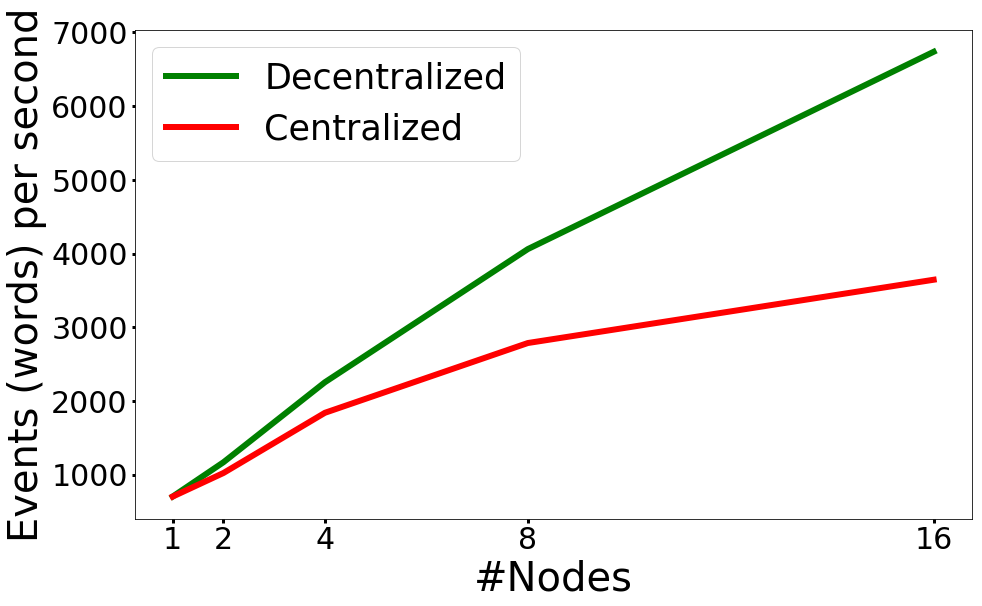
\includegraphics[scale=0.7]{throughput.png}
\end{figure}

``Decentralized'' line depicts throughput of system with distributed algorithm of change-detection while ``Centralized'' corresponds to throughput of system with single-node algorithm.

Thus, development an efficient distributed change-point detection algorithm is a practically important problem.

%\section{Dependency tracking design}
%\input {fs-lightbulbs-design}

%\section{Implementation}
%\input {fs-lightbulbs-impl}

%\section {Experiments}
%\label {fs-lightbulbs-experiments}

    
\begin{table}[h]
    \centering
    \begin{tabular}{|l||l|l|l|l|}
        \hline
         & KS & KSI & $\phi$ & $\Xi$ \\ \hline
        baseline & 8 & 9.8 & 3.6 & 7.2 \\ \hline
        1 node & 1.8 & 3.4 & 6.4 & 7.8 \\ \hline
        4 nodes & 6.2 & 7.2 & 16.8 & 14.0 \\ \hline
        8 nodes & 8.6 & 9.4 & 16.4 & 14.2 \\ \hline
        16 nodes & 13.0 & 15.0 & 14.0 & 18.4 \\ \hline
    \end{tabular}
    \caption{Experiment without changes. False detections}
\end{table}

\begin{table}[h]
    \centering
    \begin{tabular}{|l||l|l|l|l|}
        \hline
         & KS & KSI & $\phi$ & $\Xi$ \\ \hline
        baseline & 31 & 60 & 92 & 86 \\ \hline
        1 node & 27.4 & 53.8 & 75.0 & 67.6 \\ \hline
        4 nodes & 31.8 & 60.4 & 71.6 & 66.4 \\ \hline
        8 nodes & 25.2 & 60.0 & 67.0 & 61.8 \\ \hline
        16 nodes & 19.4 & 47.8 & 53.0 & 50.6 \\ \hline
    \end{tabular}
    \caption{Experiment 1. True detections}
\end{table}



\begin{table}[h]
    \centering
    \begin{tabular}{|l||l|l|l|l|}
        \hline
         & KS & KSI & $\phi$ & $\Xi$ \\ \hline
        baseline & 30 & 34 & 20 & 19 \\ \hline
        1 node & 25.2 & 25.8 & 21.8 & 23.8 \\ \hline
        4 nodes & 26.2 & 24.0 & 20.4 & 19.0 \\ \hline
        8 nodes & 27.4 & 22.2 & 17.4 & 19.0 \\ \hline
        16 nodes & 25.8 & 22.0 & 21.4 & 22.8 \\ \hline
    \end{tabular}
    \caption{Experiment 1. Errored detections (false and late)}
\end{table}

\begin{table}[h]
    \centering
    \begin{tabular}{|l||l|l|l|l|}
        \hline
         & KS & KSI & $\phi$ & $\Xi$ \\ \hline
        baseline & 0 & 4 & 16 & 13 \\ \hline
        1 node & 0.8 & 5.4 & 9.8 & 3.4 \\ \hline
        4 nodes & 3.2 & 11.2 & 12.2 & 9.8 \\ \hline
        8 nodes & 2.8 & 10.6 & 12.2 & 10.4 \\ \hline
        16 nodes & 1.4 & 5.8 & 10.8 & 8.4 \\ \hline
    \end{tabular}
    \caption{Experiment 2. True detections}
\end{table}

\begin{table}[h]
    \centering
    \begin{tabular}{|l||l|l|l|l|}
        \hline
         & KS & KSI & $\phi$ & $\Xi$ \\ \hline
        baseline & 15 & 32 & 33 & 36 \\ \hline
        1 node & 8.2 & 22.8 & 23.2 & 18.4  \\ \hline
        4 nodes & 11.6 & 25.0 & 25.6 & 20.4 \\ \hline
        8 nodes & 15.8 & 23.6 & 24.6 & 24.6  \\ \hline
        16 nodes & 13.4 & 27.6 & 27.0 & 24.4 \\ \hline
    \end{tabular}
    \caption{Experiment 2. Errored detections (false and late)}
\end{table}




%\section{Related Work}
%\input {fs-lightbulbs-related.tex}

\section {Conclusion}
\label {fs-lightbulbs-conclusion}

%In this work, we formulated and formalized a problem of dependency tracking between input and output elements in streaming dataflows. We demonstrated that state-of-the-art distributed stream processing systems face this problem in state snapshotting mechanisms~\cite{Carbone:2017:SMA:3137765.3137777, apache:storm}, the materialization of time-varying relations~\cite{Begoli:2019:OSR:3299869.3314040}, and atomic delivery of all descendants of an input item~\cite{we2018adbis}.  
In this paper we formulated and formalized a problem of distributed change-point detection in streaming dataflows. We analysed the importance of dependencies in data distribution over nodes and intoduced our version of algorithm for distributed change-point detection.

%To solve this problem, we proposed a mechanism that adopts ideas from the Apache Storm completion tracking mechanism called \acker. We extend each data item with a logical timestamp that denotes corresponding input items and track if dataflow contains elements with specific timestamps. Our solution, called \tracker, provides the following features:
%\begin{itemize}
%    \item {\bf Fine-grained tracking:} \tracker\ efficiently watches and provides notifications that system completely processed some set of input items even for individual input elements.
%    \item {\bf Cyclic graphs support:} proposed mechanism works for cyclic execution graphs, and that makes it suitable for iterative dataflows as well. 
%    \item {\bf Scalability:} we introduced a decentralized version of \tracker\ that allows a system to distribute extra network traffic between all computational units. 
%    \item {\bf Low overhead:} \tracker\ does not produce any significant performance penalty and does not affect the throughput of a distributed streaming dataflow.
%\end{itemize}

%We conducted a series of experiments and compared the proposed method with a baseline approach based on the checkpointing mechanism used in Apache Flink. We demonstrated that both centralized and decentralized implementations of \tracker\ provide lower notification latency that does not considerably degrade with an increase of a logical graph size or a cluster size. Experiments also showed that \tracker\ has lower throughput overhead in case of fine-grained tracking.

We conducted a series of experiments and compared the proposed method with a single-node methods and demonstrated that it keeps acceptable values of metrics and provides lower latency.

\bibliographystyle{abbrvurl}
\bibliography{../../bibliography/flame-stream}

\end {document}

\endinput
